\newcommand*{\EmbeddedReactiveSystems}{\begingroup

%----------------------------------------------------------------------------------------
%	Embedded Reactive Systems
%----------------------------------------------------------------------------------------
\chapter{Embedded Reactive Systems}\label{ch:embeddedReactiveSystems}
Our everyday life is supported by electronic components in almosed every aspect. A lot of these electronic components include an embedded reactive system. More than 95\% of software systems are actually embedded. \cite[cf.][2]{Oshana2013} But what are the characteristics of an embedded system and what makes it reactive? Embedded systems are the counterpart of Personal Computer (PC), notebooks and workstations. An embedded system is a computing component which is, for the user almosed invisible, embedded within electronic devices. \cite[cf.][8]{Gessler2014}. Unlike PCs, notebooks and workstations for embedded systems usually exist strict requirements for cost, energy consumption and size. The definition "a reactive system is a system that, when switched on, is able to create desired effects in its environment by enabling, enforcing or preventing events in the environment." \cite[][5]{Wieringa2003} gives an idea of how embedded systems and reactive systems merge to one powerful system. Furthermore a reactive system is defined with a number of characteristics:

\begin{itemize}
\item The system is continously interacting with its environment.
\item The process by which the reactive system interacts with its environment is usually nonterminating.
\item In its interaction with the environment, the reactive system will respond to external stimuli as and when they occur.
\item Responses of the reactive system are dependent on the current state of the system and the external stimuli that it responds to. 
\item The response consists of enabling, enforcing or prohibiting communication of behavior in its environment.
\item The behavior of a reactive system consists often of a number of interacting processes that operate in parallel. 
\item Often a reactive system must operate in real-time and is under stringent time requirements. \cite[cf.][5-6]{Wieringa2003}
\end{itemize}

\noindent So in one sentence, beeing reactive gives an embedded system the ability to interact with its environment in both directions.

\begin{floatingfigure}[r]{72mm}
\centering
\mbox{\frame{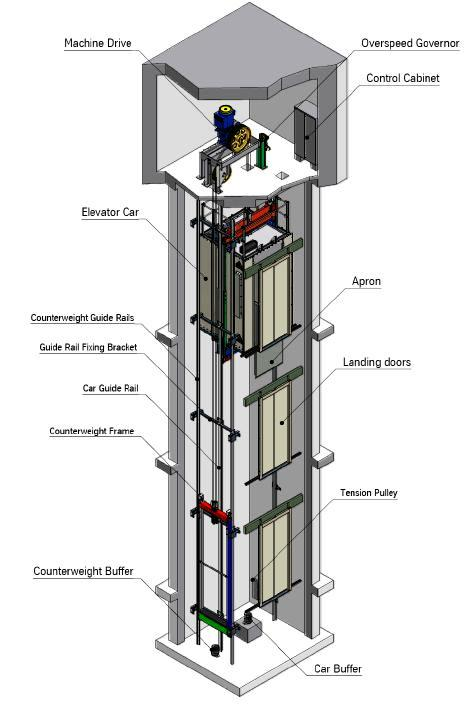
\includegraphics[width=71mm]{Images/ComponentsOfElevator.JPG}}}
\caption{Components of an elevator \cite[][]{ElectricalKnowHow2013}}
\label{fig:elevator}
\end{floatingfigure}

\noindent\\ The list of embedded reactive systems is endless. Beginning from the coffee machine in the morning, which receives the information what kind of coffee the user wants and grinds the right amount of coffee beans, over the traffic lights on the way to work which receive the request of passing the streets and stops the cars with a red signal, up to the television in the evening which receives the information of a remote control and switches the channel. 

\noindent\\ A reactive system can be divided into three basic parts. The system itself, the environment and the communication channel. The system is the processing unit which continously keeps the reactive system running. It receives messages and responds to them either internally or by sending messages. The environment is the part of the world which is relevant for the reactive system. For interacting with the environment both, the environment and the system, need an interface. And last but not least the communication channel connects these interfaces and transports the messages between the components. This could be a connection between the interface of the environment and the system as well as between several systems. \cite[cf.][11-19]{Wieringa2003} The example of an elevator gives a deeper understanding of the components of an embedded reactive system and how they do interact with each other. (Figure \ref{fig:elevator}) The environment of the system includes the elevator car and the area around the elevator. Its interface is, of course the panel of buttons inside of the car and maybe a display which displays the current floor and the direction of the car. But the interface of the environment includes much more than just a panel and a display! A number of sensors are permanently observating the environment to detect for example doorblocking objects and other safety-critical aspects. The machine drive is also part of the environment's interface. For the user of the elevator not reachable is the system placed in a control cabinet. It usually contains a hardware interface for receiving and sending messages through the communication channels. This includes the wires to the interface of the environment as well as a communication bus between two or more elevator systems to work efficiently together. The mentioned characteristics of an embedded reactive system have an direct influence on the software architecture of the system. 

%----------------------------------------------------------------------------------------
%	Software Architecture
%----------------------------------------------------------------------------------------
\section{Software Architecture}\label{sec:softwareArchitecture}
For designing a good software architecture, designers have to consider a lot of rules and principles. One major principle for every software designer is \textit{Keep It Small and Simple}! a simple software architecture is a win situation for all stakeholders. It reduces unnecessary complexity, the maintainability and expandability increases and the sourcecode usually is smaller. Another rule that should be considered for a good design is a balanced expectation of changes. Time brings changes and changes bring new requirements. A software which can be easily changed is a good software. But it is not a good idea to design a "silver bullet" which fits into any possible case. The software designer has to identify the possibility of changes to find a good balance between customizability and fixedness. A third and no less important principle is the quality. Within the designing process the software designer has to consider possible failure situations and pre-define ways to avoid or manage them. \cite[cf.][62 - 64]{Starke2015} No person would use an elevator which has no strategy implemented in case when the cables break. But does the system also need a strategy in case when the display doesn't work? Probably not. Of course this is just a surficial overview of the considerations within a design process but it gives and idea of the complexity of designing a good software architecture for embedded reactive systems. 

\noindent\\ During the designing process of an embedded reactive system software- and hadwarearchitects must work hand in hand. This is necessary because within embedded reactive systems the hardware and software take responsibility for core functions of the system. \cite[cf.][31 - 32]{Starke2015} Usually an embedded reactive system has to meet high requirements. The user of an elevator assumes that brakes are working in the right moment, that the door opens when it should open and stays closed when it should not open. Systems with that kind of constraints in time are called real-time systems. 

\newpage

\noindent\\ One concept of structuring the software of an embedded reactive system is the super loop architecture. The super loop architecture is a very common and straightforward way of implementing an embedded reactive system. Basically the super loop architecture can be divided into two phases. In the first phase the system will be initialized. After completing the initialization routines the system enters the second phase, the infinite loop. This loop contains every task and event. It processes each of them one by one and on the end it jumps back to the top of the loop where it starts to process the tasks again. A super loop architecture is only an option when the tasks and events can be processed in predictable time. Adapted variants of the super loop architecture like the power-safe super loop exist to make the task scheduling requirements more consistent with the loop execution time. \cite[cf.][24]{Oshana2013} 

\begin{floatingfigure}[r]{72mm}
\centering
\mbox{\frame{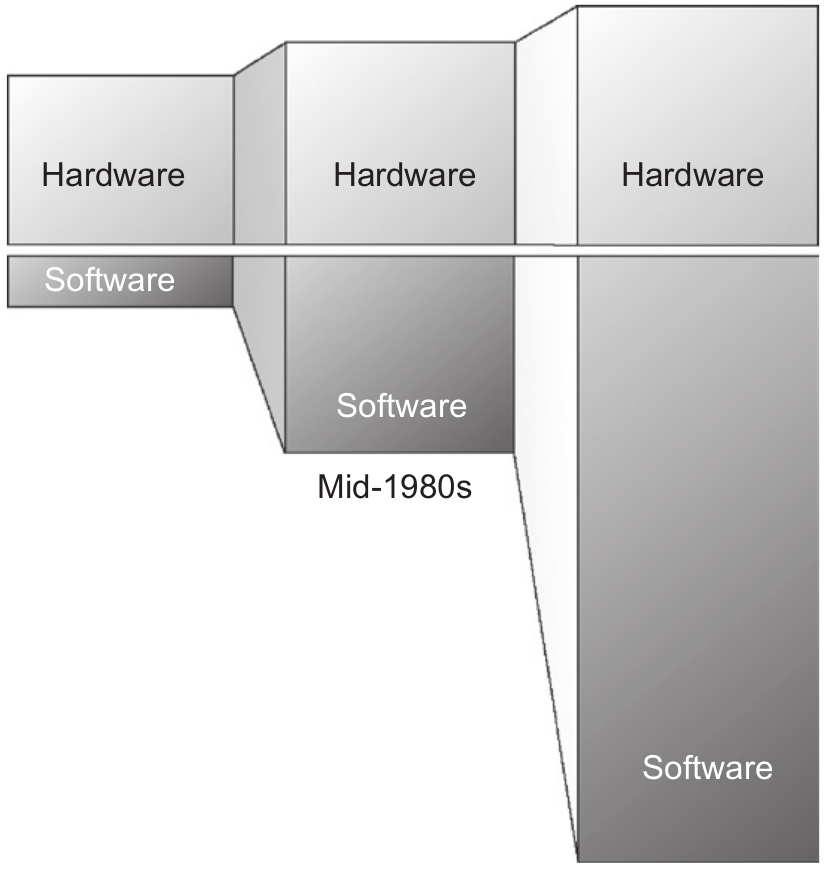
\includegraphics[width=71mm]{Images/DesignComposition.png}}}
\caption{Design composition of embedded systems \cite[][50]{Walls2012}}
\label{fig:designComposition}
\end{floatingfigure}

\noindent As example names Oshana an embedded system with an average loop time of 1ms, which needs to check a certain input only once per second. In this example it is not advisable to execute the loop 999 times before the one time comes where the input is actually relevant. In this case a delay time will be added to the super loop which reduced the execution time to an appropriate level. 

\noindent\\ In the last decades the hardware design of embedded systems has become more complex and the amount of software has increased drastically and takes up to 70 - 80\% of the total design effort. (Figure \ref{fig:designComposition}) \cite[cf.][50]{Walls2012} The embedded systems model (also known as layered software architecture) (Figure \ref{fig:embeddedSystemsModel}) is an design concept which can be used for more complex hardware and software designs. The architecture contains three main layer. An hardware abstraction layer (HAL), a system software layer and an application layer. \cite[cf.][12]{Noergaard2005} Two basic functions of the HAL are decoupling the hardware from the application and providing legible sourcecode. The I/O interface of different hardware components are usually not consistent. Every hardware component brings its own unique interface. The HAL combines and encapsulates the I/O calls within methods. These methods are used by the application layer for work with the hardware. Changes of the hardware require an update of the HAL, but the whole application layer can stay without a single change. Or in other words, the portability of the application software increases. The system software layer allows software designs with more than one process running at the same time. Responsibilities and tasks can be divided and processed in parallel. For this, the system software layer must contain at least a simple scheduler. But also operating systems including ressource- and memory management and channels for interprocess communication are possible. 

\begin{figure}[]{}
\centering
\mbox{\frame{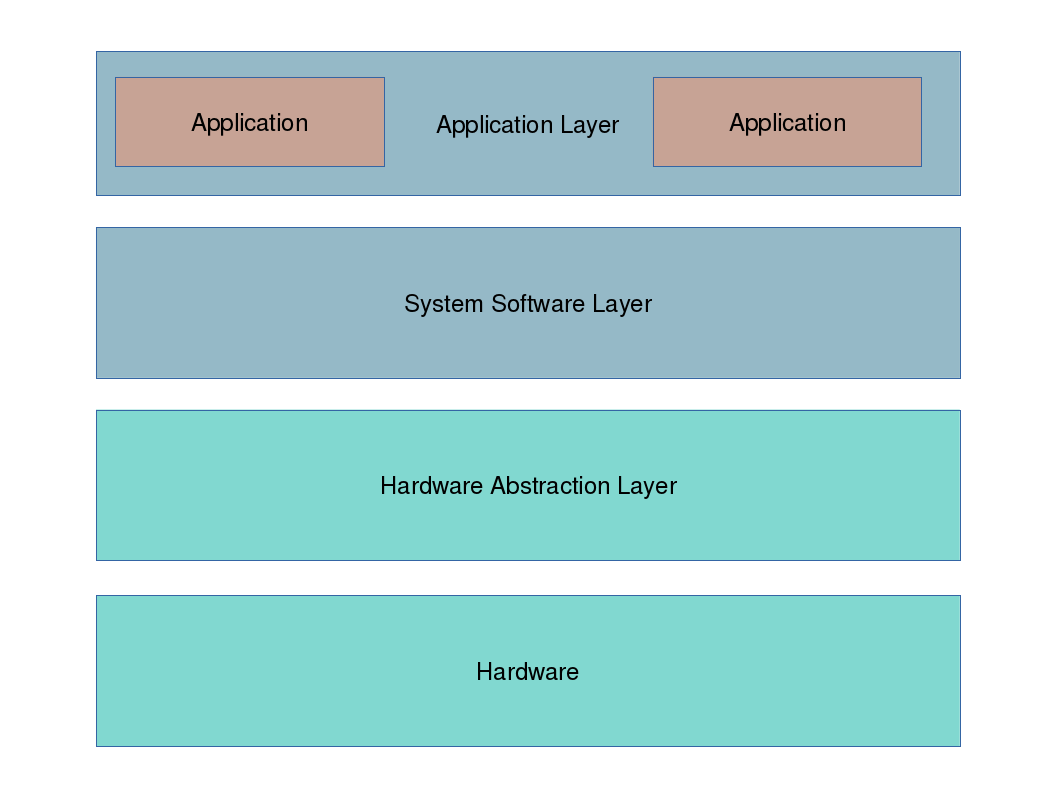
\includegraphics[width=\textwidth]{Images/EmbeddedSystemsModel.png}}}
\caption{Embedded systems model \cite[][12]{Noergaard2005}}
\label{fig:embeddedSystemsModel}
\end{figure}

\FloatBarrier

\endgroup}
